\documentclass{report}
\usepackage{graphicx}
\usepackage{titlesec}
\usepackage{mismath}
\usepackage{float}
\usepackage{hyperref}
\usepackage[letterpaper, total={6.5in, 9in}]{geometry}
\usepackage{amsmath}
\usepackage{tikzsymbols}
\usepackage{hyperref}
\hypersetup{
    colorlinks=true,
    linkcolor=blue,
    filecolor=magenta,      
    urlcolor=cyan,
    pdftitle={Overleaf Example},
    pdfpagemode=FullScreen,
    }

\urlstyle{same}
\title{%
Rocket Ramblings \\
\large Pazuki Development Notes}
\author{Het Satasiya}
\graphicspath{ {./images/} }


\newcommand{\irow}[1]{% inline row vector
  \begin{smallmatrix} (#1)\end{smallmatrix}%
}
\newcommand{\diff}[1]{\frac{\di}{\di{}t_{#1}}}

\newcommand{\cvec}[1]{\begin{bmatrix}
    #1
\end{bmatrix}}

\begin{document}


\maketitle

\pagebreak
\chapter{Rocket Math}
\section{Introduction}
This is a collection of my ramblings on how to make a rocket controlled, and hopefully land. Its going to start with the base knowledge that you need that wont be covered in a course like 9A, and an understanding of how to do basic matrix algebra ($A \times \vect{x}$, $A \times B$, $\vect{x} \cdot \vect{y}$). You also need to know how to take a derivative.

To take a rocket and control it, you first need to understand what makes it move / makes the system tick. This gives you a basis to create simulations off of, and you can linearize the equations of motion to find your system dynamics in a linearized{-}state space model. You can use a variety of control algorithms, varying from Bang{-}Bang control, PID, LQR based control, Cascade control, or Model Predictive Control (MPC). Lets get cooking.

\section{Basis}

\subsection{Reference Frames}
A reference frame is what you measure everything relative to. For example, majority of physis problems are in the `Earth-Fixed' or `Inertial' reference frame. What that means is that you have a stationary observer, and all measurements are `relative' to that stationary point. But if you were in the perspective of a moving object, then your observing a `relative' velocity and position. This creates the necessity for an equation known as the `equation of coriolis' or `something rule' depending on what dynamics professor you have. You need to use this to convert from one reference frame to another, as you have to consider the rate of angular movement around each other.  
\begin{equation} \label{eq:1} 
    \diff{i} \vect{p} =  \diff{p}\vect{p} + \omega_{p/i} \times \vect{p}
\end{equation}

I wont go into the derivation, but its written above in equation{~}\ref{eq:1}. You can use it  to convert the derivative of some position or velocity vector from one reference frame $p$ to another reference frame $i$.
\subsection{Rotation}
How you look at rotation is very important, especially when you need to maintain some form of consistency. You can represent rotation in a variety of ways, but the two that we will be considering are Euler angles, and Quaternions. Before diving into that however, your end goal needs to be to describe a rotation and rotational rate between two reference frames. The reason you cant describe rotation with just one reference frame is because of what a rotation is. If your spinning your phone, you define a `Forward', `Up', and `Side' direction to reference a rotation around. In the same way, you must mathematically define a rotation as a transformation between two reference frames. Even though a reference frame is technically `fixed' to a point (like the earth{~}fixed frame), you can `move' (in a sense) the frames to have their origins lie on top of each other to understand the rotations required to take you from one to the next. (This is the underlying principle behind Euler angles). Quaternions define rotation as a 4 dimensional vector. For further info, look \href{https://en.wikipedia.org/wiki/Quaternion}{here}.
\subsubsection{Euler Angle Rotations}
So, onto some math for rotation. Euler angle rotations can be divided up into 3 different matrices / principle rotations. 

To rotate a vector around the ${x}$ axis:
\begin{equation} \label{eq:2}
\begin{split}
\vect{x}_f &= R_x(\phi) \times \vect{x} \\
R_{x}(\phi) &= \begin{bmatrix}
    1 & 0 & 0\\
    0 & \cos{\phi} & -\sin{\phi}\\
    0 & \sin{\phi} & \cos{\phi}
\end{bmatrix}
\end{split}
\end{equation}

To rotate a vector around the ${y}$ axis:
\begin{equation} \label{eq:3}
\begin{split}
\vect{x}_f &= R_y(\psi) \times \vect{x} \\
R_y(\psi) &= \begin{bmatrix}
\cos(\psi) & 0 & \sin(\psi) \\
0 & 1 & 0 \\
-\sin(\psi) & 0 & \cos(\psi)
\end{bmatrix}
\end{split}
\end{equation}

To rotate a vector around the ${y}$ axis:
\begin{equation} \label{eq:4}
\begin{split}
\vect{x}_f &= R_z(\theta) \times \vect{x} \\
R_z(\theta) &= \begin{bmatrix}
\cos(\theta) & -\sin(\theta) & 0 \\
\sin(\theta) & \cos(\theta) & 0 \\
0 & 0 & 1
\end{bmatrix}
\end{split}
\end{equation}




And to sum it up, to rotate a vector around all axes in order, you multiply the matrices from{~}\ref{eq:2},{~}\ref{eq:3},{~}\ref{eq:4}, in that order, giving us:
\begin{equation} \label{eq:5}
    R^B_E = \begin{bmatrix}
        c\psi c\theta & c\psi s\theta  & -s\psi \\ 
        s\phi s\psi c\theta - c\phi s\theta & s\phi s\psi s\theta + c\phi c\theta & s\phi c\psi \\
        c\phi s\psi c\theta + s\phi s\theta & c\phi s\psi s\theta - s\phi c\theta & c\phi c\psi
    \end{bmatrix}
\end{equation}


\subsection{Variable names}
 We have two reference frames, a body fixed reference frame \textit{B}, and a earth fixed (inertial) reference frame \textit{E}. 

\begin{figure}[H]
\caption{Coordinate Systems, and positive notation}
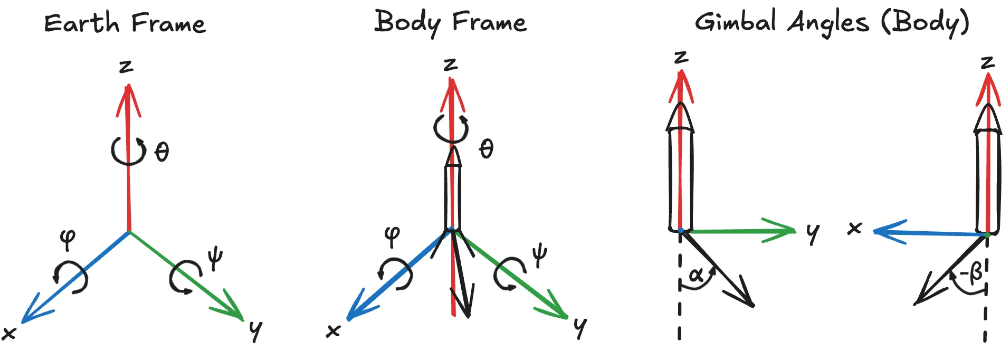
\includegraphics[width=\textwidth]{notation}
\centering
\end{figure}

Further notation / notes: $[x$, $y$, $z]$ are earth frame coordinates / positions. $[u$, $v$, $w]$ are body frame velocities in the $x$, $y$, and $z$ axes, respectively. Angular rotation is represented by $[\phi$, $\psi$, $\theta]$, with angular rates as $[p$, $q$, $r]$. Gimbal angles are represented by $\alpha$ and $\beta$, representing right hand rotations around the $x$ and $y$ axes respectively. The rotation order that we will be using is X{-}Y{-}Z. 

\section{Dynamics}

At the heart of any controller, you need to have a strong understanding of what your system dynamics are. Your system dynamics can also be thought of as the `governing equations' that determine the motion of your craft in response to external forces. 

We can define your control inputs as a force vector$\vect{F} = (f_x, f_y, f_z)$, and your control torques as $\vect{m} = (\tau_{\phi}, \tau_{\psi}, \tau_{\theta})$.

\subsection{Rocket Kinematics}
In this section we are going to find the equations that determine position wrt velocity, and rotation wrt angular rates.

$x, y, z$ are all inertial frame quantities, so you have to rotate the body frame velocities $u, v, w$. You can do that by transposing the $R^E_B$ matrix we found earlier in equation{~}\ref{eq:5}. 
%TODO: WRITE OUT COMPLETELY
\begin{equation}
    \begin{split}
        \diff{}\cvec{x\\y\\z}
        &= R^E_B \cvec{u\\v\\w}\\ 
        &={( R^B_E )}^T \cvec{u\\v\\w}
    \end{split}
\end{equation}

Rotational dynamics are harder, because you have to account for intermediate rotations. Also, by and large, your rotational velocities are pretty low, so your $R_x(\dot \phi)=R_y(\dot \psi)=R_x(\dot \theta) = I$.

\begin{equation}
    \begin{split}
        \cvec{p\\q\\r} &= R_x(\dot\phi)\cvec{\dot\phi\\0\\0} 
        + R_x(\phi)R_y(\dot\psi)\cvec{0\\\dot\psi\\0}
        + R_x(\phi)R_y(\psi)R_z(\dot\theta)\cvec{0\\0\\\dot\theta}\\
        &=\cvec{\dot\phi\\0\\0} 
        + R_x(\phi)\cvec{0\\\dot\psi\\0}
        + R_x(\phi)R_y(\psi)\cvec{0\\0\\\dot\theta}
    \end{split}
\end{equation}
\subsection{Rigid Body Dynamics}
Forces and their respective accelerations are in the inertial fixed frame, so we can use the equation of coriolis (\ref{eq:1}). $\vect{v}$ is the velocity of the object. 
\begin{equation}
    \begin{split}
        m\diff{E}\vect{v}_E &=m\left(\diff{B}\vect{v}_B + \vect{\omega}_{B/E} \times \vect{v} \right) = \vect{F} \\
        \cvec{\dot u \\ \dot v \\ \dot w} &= \cvec{rv-qw \\ pw-ru \\ qu - pv} + \frac{1}{m} \cvec{f_x \\ f_y \\ f_z}
    \end{split}
\end{equation}

Moments of inertia are written as $J_x$, $J_y$, $J_z$, along those axes (shortened from $J_{xx}, J_{yy}, J_{zz}$). If you ignore the cross products of inertia ($J_{xy}, J_{xz}$, etc), it makes your life a lot easier. And if you define your control input torques $\vect{m} = \left(\tau_{\phi}, \tau_{\psi}, \tau_{\theta} \right)$

\begin{equation}
    \cvec{\dot x \\ \dot y \\ \dot z} = 
    \cvec{ \frac{J_y - J_z}{J_x}qr 
        \\ \frac{J_z - J_x}{J_y}pr 
        \\ \frac{J_x - J_y}{J_z}pq}
    + \cvec{ \frac{1}{J_x} \tau_{\phi} \\ 
             \frac{1}{J_y} \tau_{\psi} \\ 
             \frac{1}{J_z} \tau_{\theta}}
\end{equation}

And thats a wrap for our dynamics \dSmiley.

\chapter{Control}
Heres the fun part, which is trying to control your system. There are so many ways to do it, but lets start with some more important definitions. The thing that you want to control is called your `system' or `plant'. Whatever variables that you can apply to modify your system are your `control inputs'. And the different quantities of your system that you can measure and want to control are called your `states'.

\section{Control Algorithms}
Now that we have that out of the way, lets define a little toy system to learn about everything here. Lets start with our equations of motion.

We can define our states as our vertical position $y$ and our vertical velocity $v$. Our control input is a force in the y{-}axis, $F$. The object has a mass $m = 1kg$, and an acceleration from gravity $g = 9.81 m/s^2$ on it. 

\begin{equation}
    \vect{x} = \cvec{y \\ v},
    \vect{\dot x} = \cvec {\dot y \\ \dot v},
    \vect{u} = \cvec{F}
\end{equation}

\begin{equation} \label{simple_eom}
    \begin{split}
        y & = vt \\
        v & = \left( \frac{F}{m} \right) t - g * t    
    \end{split}
\end{equation} 

That should be enough to make a basic simulation of our object using some python or MATLAB and Simulink depending on what you want to do. 

\subsection{PID Control}
Lets create a simple controller, and explore what driving a system to a state looks like and how modifying relatively simple variables changes the response time.


\end{document}


% TODO: Dynamics derivation, cant be that bad 
% Going over PID and LQR control
% Start with the 